\vspace{-1ex}
%%%%%%%%%%%%%%%%%%% Section 8 %%%%%%%%%%%%%%%%%%%%%%%
\section{Approximate Optimal Backbones}
\label{sec-approx}

Theorem~\ref{thm-hardness} tells us that
\abd is inherently hard to approximate; yet
not all is lost. We
study its {\em fixed-parameter approximability}~\cite{marx2008parameterized}.
Our first result considers a practical
assumption that real-world networks pertain to
small $|\A|$.

\stitle{Fixed-parameter approximability}.
An instance of a parameterized
optimization problem ${\cal I}$ is a triple $(x, k, C)$,
with an input of size $|x|$ structured by a parameter $k$, and an objective function $C$ (to be minimized).
We say the problem 
${\cal I}$ is {\em fixed-parameter $\alpha$-approximable} ($\alpha\in[0,1]$), if the following condition holds:

\sstab
(1) there exists a function $f$ and an algorithm such that for any instance $(x,k)$ of ${\cal I}$,
it takes $O(f(k)\cdot|x|^c)$ time to
find a solution $y$, where $c$ is a constant; and

\sstab
(2) $C(y)\leq (1+\alpha) * C(y^*)$,
where $y^*$ is the optimal solution.

\vspace{.5ex}
In practice, such an algorithm is feasible if
$k$ is small. In the case that
$\A$ is small
for $G$, we parameterize \abd with
$l$ = $\max_{v\in V}|\A(v)|$ ($l\geq 1$).
We have the following result.


\begin{theorem}
\label{theo-approx}
\abd is fixed-parameter $2$-approximable with fixed
$l$; more specifically, there exists an algorithm
that
(1) guarantees an Lagrangean-preserving 2-approximation,
\ie it computes a backbone $T$ such that
\[
C(E_T)+2\cdot I(\bar{V_T})\leq 2\cdot\cost(T^*)
\]
where $T^*$ is the optimal attribute-driven backbone;
and (2) runs in $O((2^{l}-1)|E|\log |V|)$ time.
\end{theorem}

As a constructive proof for Theorem~\ref{theo-approx},
we next introduce the algorithm with the optimally guarantees.


\subsection{Approximation Algorithm}

Our first algorithm, denoted as \approxabd,
computes attributed backbones with Lagrangean preserving 2-approximation in polynomial time when $\A$ is small.

\stitle{Overview}. In a nutshell, the algorithm \approxabd
dynamically maintains a set of ``active'' clusters $\P$
of nodes (initialized as singletons from $V_I$), where
each cluster induces a spanning tree that
has potential to be a subtree of an optimal backbone.
It iteratively grows each active cluster $P\in \P$ with
a class of {\em affinitive edges} $E_A(P)$,
where each affinitive edge $e\in E_A(P)$
(a) contains only one end node in $P$, and
(b) carries a
distinct set of affinitive attributes $F(e)$.
In this process, \approxabd verifies two predicates
that can grow the backbone:
\bi
\item \textbf{IsGrow}: Can any cluster be expanded with
an affinitive edge (remain `active')?
\item \textbf{IsMerge}: Can any two clusters be merged?
\ei

The conditions are determined by a set of
auxiliary values defined on $C$ and
$E_A(C)$.
The growth and merge process terminates when there is no
active cluster in $\P$,
\ie a largest cluster is constructed and can no longer be
expanded. The attributed backbone is then induced
from the largest cluster.

\vspace{.5ex}
We start with an outline of~\approxabd, followed by
the detailed procedures and performance analysis.


\stitle{Algorithm}.
The algorithm~\approxabd (illustrated in Fig.~\ref{fig:approxABD})
dynamically maintains clusters $\P$, and
for each cluster  $P\in \P$,
it bookkeeps
(1) a status flag indicating whether it's
``active'' or ``inactive'';
(2) three types of values to control the updates
of $C$, including a {\em surplus value} $s(P)$ = $\sum_{v\in P\cap V_I}I(v)$, a {\em moat value} $y(P)$ (initialized as $0$), and
for each affinitive edge $e\in E_A(P)$, a surplus value
$s(e)$ = $C(e, F(e))$.
In addition, it maintains two priority queues
of $\P$: $\Q_P$ that indexes $\P$ by an
ascending order of $s(P)$,
and $\Q_E$ that prioritize\reviseS{s} $\P$ by
ascending order of
$\min_{e\in E_A(P)}s(e)$, \ie
the smallest surplus value in the
affinitive edge set $E_A(P)$.

%%%%%%%%%%%%%%%%%%%%%%%%%%%%%%%%%%%%%%%%
\begin{figure}[tb!]
%\vspace{-1ex}
\begin{center}
{\small
\begin{minipage}{3.36in}
\myhrule
\vspace{-1ex}
%%%%%%%%%%%%%%%%%Algorithm \paragfd%%%%%%%%%%%%
\mat{0ex}{
{\bf Algorithm}~\approxabd\\
\sstab {\sl Input:\/}
\= graph $G$=$(V,E,F_A)$, cost model $C$, interested nodes $V_I\subseteq V$.\\
{\sl Output:\/} An attributed backbone $T = (V_T,E_T,F_T)$.\\
%%%%%%%%%%%%%%%%%%%%%%%%%%%%%%%%%%%%%%%%
\bcc \hspace{3.6ex}\= Initializes $\P$, $\Q_E$, $\Q_P$; $\updateAE(\P)$; backbone $T$:=$\emptyset$; \\
\icc\> \While there is an active cluster in $\P$ \Do \\
\icc\> \hspace{2ex} $(e_{\min}, P_v, P_v')$ := $\kw{topEdge(\P, \Q_E)}$; \\
\icc\> \hspace{2ex} \If \isgrow($\P$) = \kw{true} \Then /* {\em grow the clusters in $\P$ } */\\%/*
\icc\> \hspace{4ex} update $s(e_{\min})$; \\
\icc\> \hspace{4ex} \If $\ismerge(e_{\min}, P_v, P_v')$ = \kw{true} \Then \\
\> /* {\em merge clusters and update affinitive edges for the new cluster} */\\
\icc\> \hspace{6ex} $\merge(P_v, P_v', \P, T)$;  $\updateAE(\P)$; \\
\>  /* {\em grow clusters with
their best affinitive edges} */\\
\icc\> \hspace{4ex} \Else $\grow(\P, \Q_E)$;  \\
\> /* {\em deactivate the clusters in $\P$ } */\\
\icc\> \hspace{2ex} \Else \deactivate$(\kw{topCluster(\P,\Q_P)})$;\\
\icc\> \refine($T$); /* {\em prune edges to ensure tree structure} */ \\
\icc\> \Return $T$;  \\
}
\vspace{-3ex}
\myhrule
\end{minipage}
}
\end{center}
\vspace{-2ex}
\caption{Algorithm~\approxabd} \label{fig:approxABD}
\vspace{-3ex}
\end{figure}

\vspace{.5ex}
Algorithm~\approxabd has the following three phases.

\etitle{Initialization}.
\approxabd initializes the active clusters $\P$ as
follows: for each node of interests $v\in V_I$,
there is a singleton $P_v\in \P$, where
$s(P_v)$ = $I(v)$ and $y(P)$ = $0$.
It then invokes a procedure~\updateAE (line~1)
to initialize the affinitive edges for
each cluster $P_v\in \P$.
Specifically, for each edge $e$=$(v,v')$ adjacent to
$v$, $E_A(P_v)$ contains a set of
affinitive edges $e$, each carries a distinct set of
affinitive attributes $F(e)\subseteq \A(v)\cap\A(v')$.
Finally, it updates $s(e)$ = $C(e, F(e))$.
The queues $\Q_E$ and $\Q_P$ are initialized
accordingly.

\etitle{Clustering}.
It then iteratively performs the following (lines~2-9).
It first fetches a triple $(e_{\min}, P_v, P_v')$, where
$e_{\min}$ refers to an affinitive edge $(v,v')$ of $P_v$ with the
smallest surplus value $s(e)$, $P_v$ and $P_v'$ are two clusters
connected by $e_{\min}$. It then verifies
the condition \isgrow holds, which indicates that the
active clusters can be expanded to cover more interested nodes.
Specifically, \approxabd tracks, for each
cluster $P$, a set of all the ``childern''  clusters $\{P_1, \ldots, P_m\}$ that were merged into $P$.
The condition \isgrow then tests
whether for every $P\in \P$,
$\Sigma^n_{i=1}$ $y(P_i)< s(P)$,
and performs the following:

\sstab
(a) If all the clusters $\P$ can be
expanded and contribute to the growth
of backbone $T$, \approxabd verifies 
two cases below that may lead to larger clusters:

\tbi
\item Clusters $P_v$ and $P_v'$ can be merged, verified by
the condition \ismerge (lines 6-7). More specifically, \ismerge tests whether
$s(e_{\min}) = 0$.
If so, it invokes procedure \merge to
construct a new cluster $P'$ = $P_v\cup P_v'$,
set $y(P')$ = $0$,
deactivate $P_v$ and $P_v'$, and
add the affinitive edge $e_{\min}$ to
$T$ %as a new backbone edge 
(not shown).
It then constructs new affinitive edges for $P'$
and update $\Q_E$ and $\Q_P$ (line~7) for the next
round of clustering.

\vspace{.5ex}
\item Otherwise, it invokes a procedure~\grow to expand the clusters (line~8).
For each cluster $P\in \P$, it enlarges $P$
with its affinitive edge having the smallest $s(e)$.
It also enlarges $y(P)$ for all the clusters
$P$ at a same rate until \isgrow is violated.
\ei

\sstab
(b) If there
exists a cluster that can not be enlarged
and contribute to $T$, it deactivates the cluster.
This is simply performed by selecting the
top cluster in $\Q_P$ (line~9),
which has an affinitive edge $e$ with the smallest $s(e)$
among all affinitive edges of all the active clusters.


\etitle{Refinement}.
Once there is no active cluster in $\P$, \approxabd induces subgraph $T$ that consists of affinitive edges 
added in the merge phase (lines 6-7). It then invokes
procedure~\refine to prune $T$. 

\begin{example}
\label{exa- ABD running}
Fig. \ref{fig:backbonemerge} illustrates the moment that two clusters
$C_1$ that contains $v_1$
and $C_2$ that contains $v_2$
(Fig.~\ref{fig:backboneex}) are
 merged to a new cluster $C_4$ via
 an affinitive edge
$e$, with affinitive attribute ${\texttt{location}}$.
The condition \isgrow first verifies
that the current clusters
$C_1$ and $C_2$ can still grow.
It then identifies all the affinitive
edges of $C_4$, including
three affinitive edges $e_1$-$e_3$.
As $C_4$ and $C_3$ (that contais
$v_3$) ``meets'',
\ismerge is tested to verify
whether $s(e_3)$ satifies
the merge condition.
If so, a new cluster that
merges $C_4$ and $C_3$ is constructed,
inducing $T$ that contains
edges $e$ and $e_3$ carrying
{\texttt{gender}}.
\end{example}


\subsection{Performance Analysis}

The algorithm~\approxabd guarantees to terminate:
there are at most $|V|$ clusters, and each round
either deactivates a cluster that are no longer
activated, or reduces a cluster by \merge.
%%%%%%%%%%%%%%%%%%%%%%%%%%%%%%%%%%%%%%%%%%%%
We next provide an analysis for the approximability and
time cost of the algorithm~\approxabd.

\vspace{1ex}
\stitle{Approximability}.
We next introduce the two predicates \isgrow and \ismerge,
and clarify the approximation guarantee of
\approxabd. To clarify these, we
consider a multigraph $\G$ obtained by
running procedure~\updateAE over every node
$v\in V$, which creates $2^{|\A(v)\cap\A(v')|}$
affinitive edges between two nodes $v$ and $v'$,
each carries a subset of $\A(v)\cap\A(v')$.
We observe that \abd is equivalent to
computing a {\em prize collecting Steiner tree} problem
over $\G$, which has the following
dual of the Primal \abd over $\G$ (Section~\ref{sec-pre}):
\begin{equation*}
\label{eqn_PCST_dual}
\begin{alignedat}{3}
&\textrm{maximize} \quad &&\sum_{S \subseteq \V -\{r\}}y_S\\
&\textrm{subject to} \quad &&\sum_{S: e \in \delta(S)}y_S \leq c_e \quad &&\forall e \in \E,\\
&\quad &&\sum_{S \subseteq U}y_S \leq \pi(U) \quad &&\forall U \subseteq \V,\\
&\quad &&y_S \geq 0 \quad &&\forall S \subsetneq \V,\\
&\quad && G = (\V, \E)
\end{alignedat}
\end{equation*}

We take a closer look at the growth stage
(lines~2-9). Observe that the moat value
$y(P)$ can be viewed as the dual variables.
A cluster $P$ is ``active'' if and only if it has a
positive surplus. In each round of the growth stage, \approxabd uniformly raises moat values for each
cluster $P$, while decreasing its corresponding surpluse $s(P)$ to pay for the increases, until either edge constraint becomes tight or the cluster constraint becomes tight as constraints of Dual.

These correspond to the two conditions below:
%\warn{link the conditions to constraints.}

\begin{itemize}
\item the condition \isgrow tests
whether all the active components can keep growing or not. If ${\sum_{S \subseteq U}y_S < \pi(U)}$ (${\forall U \subseteq V }$), $\isgrow(P)$ is true, and false otherwise;
\item the condition \ismerge tests whether any edge $e$ (${\forall e \in E}$) satisfies: ${C(e, F(e)) = \sum_{S: e \in \delta(S)}y_S}$.
\end{itemize}
Algorithm~\approxabd then simulates a \GW scheme to
compute a prize-collecting Steiner tree
over $\G$. The approximation follows from
an approximation preserving reduction
from the instance of \abd problem to
the prize-collecting Steinter tree
problem over $\G$. It has been proven to have an Lagrangean-preserving 2-approximation \cite{feofiloff2010note,chudak2004approximate} on the Prize-collecting Steiner tree problem.



\begin{figure}[tb!]
%\vspace{-1ex}
\centering
\centerline{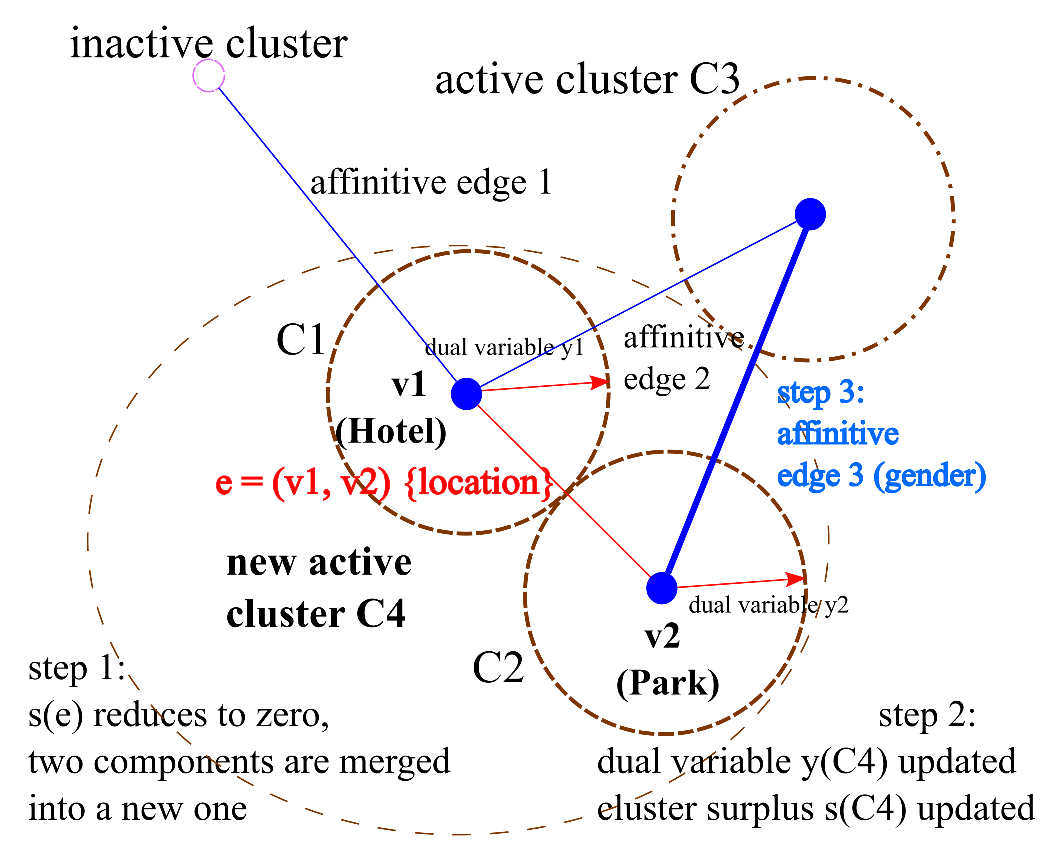
\includegraphics[scale=0.38]{./fig/runningExampleABD_v2.eps}}
\vspace{-1ex}
\caption{Dynamic clustering with affinitive edges}
\label{fig:backbonemerge}
\vspace{-3ex}
\end{figure}



\stitle{Time cost}.
It takes in total $O(|V|+|E|)$ time to initialize
the computation. In the growth phase (lines~2-9),
the total number of processed edges and connected clusters
is at most $(2^l-1)|E|$; and each processing
takes $O(\log|V|)$ time by accessing priority queues
$\Q_E$ and $\Q_P$. \merge and \refine take
$O(|V|)$ time. The total time cost
is thus
$O((2^l-1)|E|\log|V|)$. Putting these together, Theorem~\ref{theo-approx}
follows.








